\documentclass[a4paper]{jpconf}
\usepackage{graphicx}

\bibliographystyle{LaTexTemplates/BibTeX/iopart-num/iopart-num}


\begin{document}
\title{First measurements of muon production rate using a novel pion capture system at MuSIC}

\author{S Cook$^1$, M Wing$^1$, A Sato$^2$ and Y Kuno$^2$}

\address{$^1$Department of Physics and Astronomy, University College London, Gower Street, London WC1E~6BT, UK}
\address{$^2$Department of Physics, Graduate School of Science, Osaka University.}

\ead{scook@hep.ucl.ac.uk}

\begin{abstract}
The MuSIC (Muon Science Innovative Channel) beam line at RCNP (Research Centre for Nuclear Physics, Osaka) will be the most intense source of muons in the world. A proton beam is incident on a target and, by using a novel capture solenoid, guides the produced pions into the beam line where they subsequently decay to muons. This increased muon flux will allow more precise measurements of cLFV (charge Lepton Flavour Violation) as well as making muon beams more economically feasible. Currently the first 36$^{\circ}$ of solenoid beam pipe have been completed and installed for testing with low proton current of 1nA. Measurements of the total particle flux and the muon life time were made. The measurements were taken using thin plastic scintillators coupled to MPPCs (Multi-Pixel Photon Counter) that surrounded a magnesium/copper  stopping target. The scintillators were used to record which particles stopped and their subsequent decay times.
\end{abstract}    


\begin{quotation}
    \begin{center}
        Contribution to:
        NUFACT 11, XIIIth International Workshop on Neutrino Factories, Super beams and Beta beams, 1-6 August 2011, CERN and University of Geneva
        (Submitted to IOP conference series)
    \end{center}
\end{quotation}



\section{Introduction}
The Muon Science Innovative Channel (MuSIC) is a muon beam line being built at the Research Centre for Nuclear Physics (RCNP) in Osaka, Japan. It uses a strong, 3.5~T, magnetic field to create nearly 2$\pi$~Sr pion capture region. Compared to existing methods of muon production MuSIC's pion capture solenoid has a significantly higher acceptance and so is has a much higher proton to muon efficiency.

The second stage of the system is a 180$^{\circ}$, 3m diameter, transport solenoid that allows the pions to decay to muons, increasing the total flux. The transport solenoid also acts as a momentum selector and has a dipole field of 0.04~T that allows selection of either positive or negative particles. The system is based upon the muon production system of the COMET project and is a prototype of it. 

Once commissioning is complete MuSIC will be used for a variety of science and R\&D projects, these include development of the muon momentum matching and injecting system required to use an FFAG as a muon storage ring. Other areas of research will include precision measurements of the rate of $\mu \rightarrow eee$ and use in muon spin rotation ($\mu$SR).

\section{Overview}
The MuSIC experiment uses the 400~MW proton beam supplied from the RCNP's cyclotron. It provides 400~MeV protons with a maximum current of 1~$\mu$A. The beam is aimed at a graphite target situated at the centre of a 3.5~T superconducting capture solenoid. Backwards travelling pions are captured and channeled into a 3~m diameter 2~T transport solenoid where they will decay to muons prior to use. Using dipole magnets the muon charge and momentum can be selected using the transport solenoid allowing direct control of the beam profile.

Commissioning of MuSIC began in 2009 with the installation of the capture solenoid and first 36$^{\circ}$ of the transport solenoid at the Research Centre for Nuclear Physics (RCNP) in Osaka, Japan. Figure~\ref{fig:MuSIC_schematic} shows the current construction. The cooling of the superconducting solenoids and protons successfully delivered in 2010. 

MuSIC has now finished three successful runs at the RCNP using a reduced proton beam of between 0.6~pA and 10~nA. The three runs were in July 2010, February 2011 and June 2011. Once measurements of the background neutron flux have been made then MuSIC will be cleared to begin ramping to the higher 1~$\mu$A current.    

\begin{figure}[htbp]
    \centering
        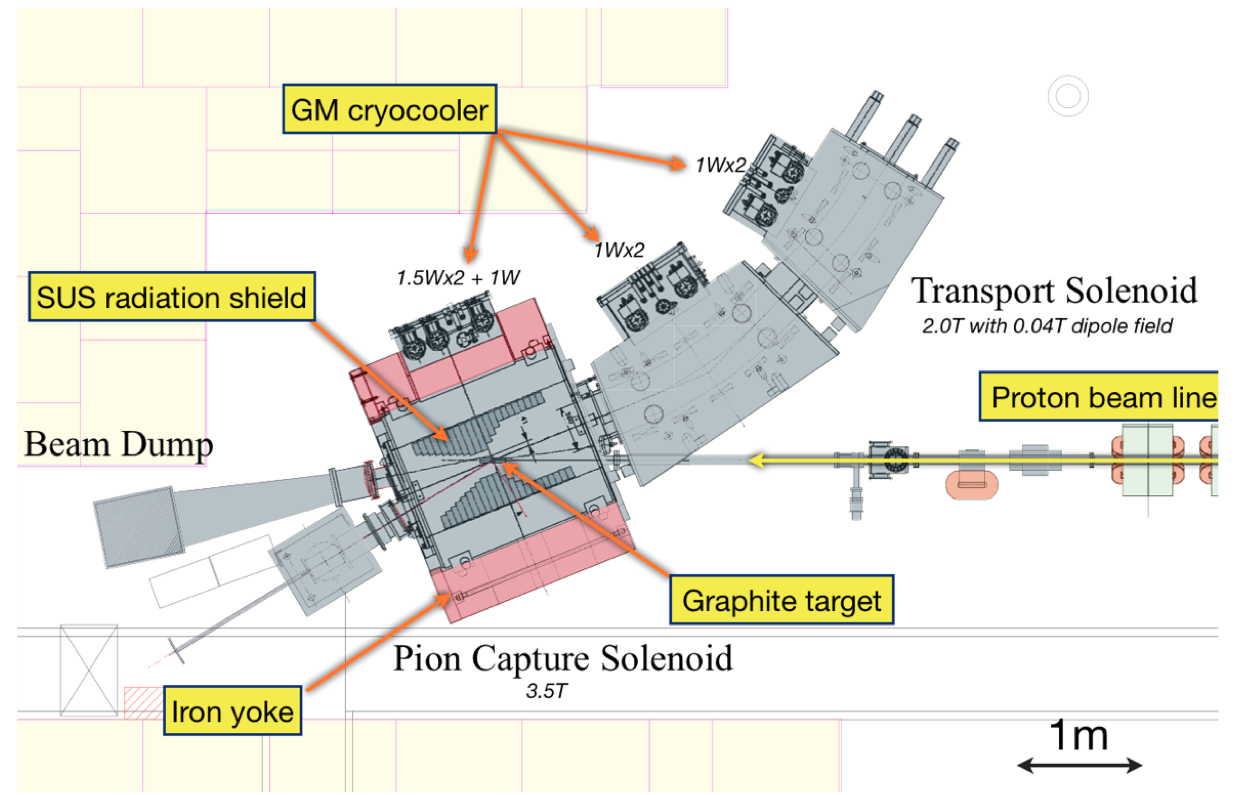
\includegraphics[height=7.5cm]{images/MuSIC_current_schematic.png}
    \caption{Schematic of the current status of the MuSIC pion production system.}
    \label{fig:MuSIC_schematic}
\end{figure}


\section{Measurement of muon flux}
\subsection{Measurement of the muon lifetime}
In order to establish both the presence of muons in the beam and their flux the muon lifetime was measured. The experimental set up consisted of two plastic scintillators ($400\times 50\times 3.5$mm$^3$) on either side of a copper stopping target ($370\times 80\times 6$mm$^3$). This arrangement was held in place using an aluminium surround positioned at the end of the beam pipe. 

To measure the lifetime a simple trigger system was devised to detect stopped muons and then measure the time taken for the decay electron to be emitted. A gate of 3~$\mu$s was used to look for the decay electron. The logic for detection of a muon was a hit in the front scintillator but not the rear whilst an electron was taken as a single hit in either the front or the read scintillator. 

A multi-TDC was used to time every hit that triggered only one of the scintillators after the initial muon. Readout from the scintillators was done using MPPCs which have an output signal proportional to the number of photons that strike their surface. MPPCs were used instead of traditional PMTs as they work well in strong magnetic fields and can be directly mounted to the scintillator without light guides, which reduces the cost and complexity of the system. 

The beam supplied during the measurement was a 6~pA proton beam at 392~MeV. This exceeds the pion production threshold.

A preliminary analysis has been carried out in which two exponential curves have been fitted to the data. The fit was composed of three functions: a fixed value that accounted for the constant background and two exponential terms that accounted for the muon decay time in copper and a free electron. The measurement of the muon in copper was 169$\pm$17~ns whilst the measured value for a free muon is 2127$\pm$20~ns. As can be seen in table~\ref{tab:muon_halflifes} the measured value for a free muon does not agree with the value in reference \cite{Pdg2010} but does agree with the mean of the values for a free muon and a muon in a plastic scintillator (taken to be predominately carbon as described in \cite{Suzuki1987muonCapture}). This implies a final beam current of 3$\times 10^8$ muon s$^{-1}$ should be achievable. 


\begin{table}
    \begin{center}  
        \lineup
    \begin{tabular}{l l l l l l}
        \br
        Material             & Measured (ns)    & Previous (ns)        & Ref \cr
        \mr                                                           
        Plastic scintillator & 2127  $\pm$ 20 & 2026.3   $\pm$ 1.5   & \cite{Suzuki1987muonCapture} \cr
        Free Muon            & 2127  $\pm$ 20 & 2197.034 $\pm$ 0.021 & \cite{Pdg2010}     \cr
        Copper               &  169  $\pm$ 17 &    164.0 $\pm$ 1.6   & \cite{Suzuki1987muonCapture} \cr
        \br
    \end{tabular}
    \end{center}
    \caption{Muonic decay times. The measured value for plastic scintillator and a free muon is the same as we did not have the data needed to resolve these two components. The }
    \label{tab:muon_halflifes}
\end{table}

\begin{figure}[htbp]
    \centering
        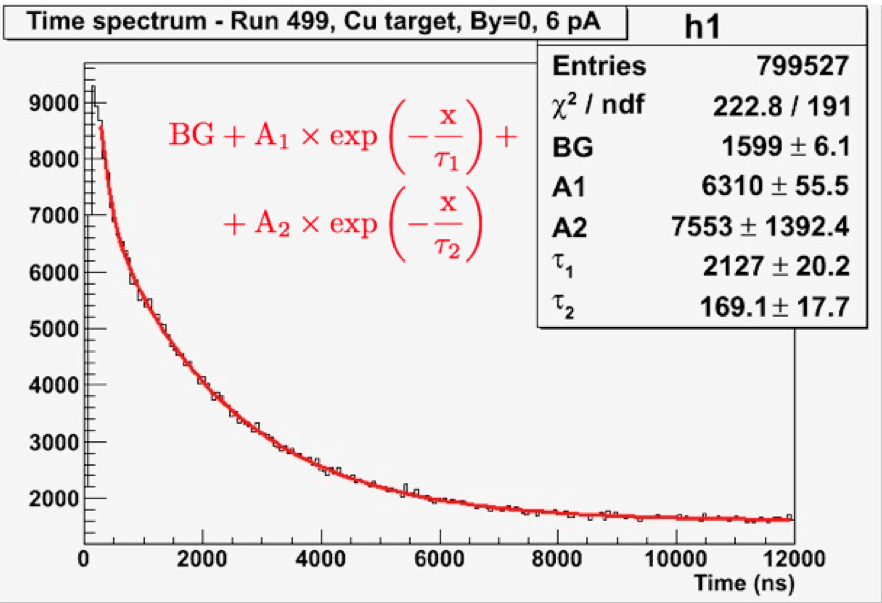
\includegraphics[height=7.5cm]{images/muon_decay.png}
\caption{Decay time for muons stopped in a copper target. Fitted with two exponentials, corresponding to the free muon decay time and the combination of muons stopping in copper and scintillator (see )}
    \label{fig:muon_decay}
\end{figure}


\section{Prospects}
At time of writing a fourth beam time is being planned to measure the background neutron flux in order to establish whether further shielding is required. Assuming a successful run then beam time is scheduled for early 2012 in order to begin using higher beam currents with the ultimate aim of measuring the highest intensity muon beam in the world. Beyond that it is hoped that the commissioning can be completed in the next 4 years 
\section{Conclusion}

\section*{References}
\bibliography{nufact}
\end{document}
















